%%%%%%%%%%%%%%%%%%%%%%%%%%%%%%%%%%%%%%%%%
% Wenneker Article
% LaTeX Template
% Version 2.0 (28/2/17)
%
% This template was downloaded from:
% http://www.LaTeXTemplates.com
%
% Authors:
% Vel (vel@LaTeXTemplates.com)
% Frits Wenneker
%
% License:
% CC BY-NC-SA 3.0 (http://creativecommons.org/licenses/by-nc-sa/3.0/)
%
%%%%%%%%%%%%%%%%%%%%%%%%%%%%%%%%%%%%%%%%%

%----------------------------------------------------------------------------------------
%	PACKAGES AND OTHER DOCUMENT CONFIGURATIONS
%----------------------------------------------------------------------------------------
\documentclass[10pt, a4paper, twocolumn]{article} % 10pt font size (11 and 12 also possible), A4 paper (letterpaper for US letter) and two column layout (remove for one column)
\usepackage{placeins}
\usepackage{multirow}
\usepackage{amsmath}
\newcommand{\comment}[1]{}
%%%%%%%%%%%%%%%%%%%%%%%%%%%%%%%%%%%%%%%%%
% Wenneker Article
% Structure Specification File
% Version 1.0 (28/2/17)
%
% This file originates from:
% http://www.LaTeXTemplates.com
%
% Authors:
% Frits Wenneker
% Vel (vel@LaTeXTemplates.com)
%
% License:
% CC BY-NC-SA 3.0 (http://creativecommons.org/licenses/by-nc-sa/3.0/)
%
%%%%%%%%%%%%%%%%%%%%%%%%%%%%%%%%%%%%%%%%%

%----------------------------------------------------------------------------------------
%	PACKAGES AND OTHER DOCUMENT CONFIGURATIONS
%----------------------------------------------------------------------------------------

\usepackage[english]{babel} % English language hyphenation

\usepackage{microtype} % Better typography

\usepackage{amsmath,amsfonts,amsthm} % Math packages for equations

\usepackage[svgnames]{xcolor} % Enabling colors by their 'svgnames'

\usepackage[hang, small, labelfont=bf, up, textfont=it]{caption} % Custom captions under/above tables and figures

\usepackage{booktabs} % Horizontal rules in tables

\usepackage{lastpage} % Used to determine the number of pages in the document (for "Page X of Total")

\usepackage{graphicx} % Required for adding images

\usepackage{enumitem} % Required for customising lists
\setlist{noitemsep} % Remove spacing between bullet/numbered list elements

\usepackage{sectsty} % Enables custom section titles
\allsectionsfont{\usefont{OT1}{phv}{b}{n}} % Change the font of all section commands (Helvetica)

%----------------------------------------------------------------------------------------
%	MARGINS AND SPACING
%----------------------------------------------------------------------------------------

\usepackage{geometry} % Required for adjusting page dimensions

\geometry{
	top=1cm, % Top margin
	bottom=1.5cm, % Bottom margin
	left=2cm, % Left margin
	right=2cm, % Right margin
	includehead, % Include space for a header
	includefoot, % Include space for a footer
	%showframe, % Uncomment to show how the type block is set on the page
}

\setlength{\columnsep}{7mm} % Column separation width

%----------------------------------------------------------------------------------------
%	FONTS
%----------------------------------------------------------------------------------------

\usepackage[T1]{fontenc} % Output font encoding for international characters
\usepackage[utf8]{inputenc} % Required for inputting international characters

\usepackage{XCharter} % Use the XCharter font

%----------------------------------------------------------------------------------------
%	HEADERS AND FOOTERS
%----------------------------------------------------------------------------------------

\usepackage{fancyhdr} % Needed to define custom headers/footers
\pagestyle{fancy} % Enables the custom headers/footers

\renewcommand{\headrulewidth}{0.0pt} % No header rule
\renewcommand{\footrulewidth}{0.4pt} % Thin footer rule

\renewcommand{\sectionmark}[1]{\markboth{#1}{}} % Removes the section number from the header when \leftmark is used

%\nouppercase\leftmark % Add this to one of the lines below if you want a section title in the header/footer

% Headers
\lhead{} % Left header
\chead{\textit{\thetitle}} % Center header - currently printing the article title
\rhead{} % Right header

% Footers
\lfoot{} % Left footer
\cfoot{} % Center footer
\rfoot{\footnotesize Page \thepage\ of \pageref{LastPage}} % Right footer, "Page 1 of 2"

\fancypagestyle{firstpage}{ % Page style for the first page with the title
	\fancyhf{}
	\renewcommand{\footrulewidth}{0pt} % Suppress footer rule
}

%----------------------------------------------------------------------------------------
%	TITLE SECTION
%----------------------------------------------------------------------------------------

\newcommand{\authorstyle}[1]{{\large\usefont{OT1}{phv}{b}{n}\color{DarkRed}#1}} % Authors style (Helvetica)

\newcommand{\institution}[1]{{\footnotesize\usefont{OT1}{phv}{m}{sl}\color{Black}#1}} % Institutions style (Helvetica)

\usepackage{titling} % Allows custom title configuration

\newcommand{\HorRule}{\color{DarkGoldenrod}\rule{\linewidth}{1pt}} % Defines the gold horizontal rule around the title

\pretitle{
	\vspace{-30pt} % Move the entire title section up
	\HorRule\vspace{10pt} % Horizontal rule before the title
	\fontsize{32}{36}\usefont{OT1}{phv}{b}{n}\selectfont % Helvetica
	\color{DarkRed} % Text colour for the title and author(s)
}

\posttitle{\par\vskip 15pt} % Whitespace under the title

\preauthor{} % Anything that will appear before \author is printed

\postauthor{ % Anything that will appear after \author is printed
	\vspace{10pt} % Space before the rule
	\par\HorRule % Horizontal rule after the title
	\vspace{20pt} % Space after the title section
}

%----------------------------------------------------------------------------------------
%	ABSTRACT
%----------------------------------------------------------------------------------------

\usepackage{lettrine} % Package to accentuate the first letter of the text (lettrine)
\usepackage{fix-cm}	% Fixes the height of the lettrine

\newcommand{\initial}[1]{ % Defines the command and style for the lettrine
	\lettrine[lines=3,findent=4pt,nindent=0pt]{% Lettrine takes up 3 lines, the text to the right of it is indented 4pt and further indenting of lines 2+ is stopped
		\color{DarkGoldenrod}% Lettrine colour
		{#1}% The letter
	}{}%
}

\usepackage{xstring} % Required for string manipulation

\newcommand{\lettrineabstract}[1]{
	\StrLeft{#1}{1}[\firstletter] % Capture the first letter of the abstract for the lettrine
	\initial{\firstletter}\textbf{\StrGobbleLeft{#1}{1}} % Print the abstract with the first letter as a lettrine and the rest in bold
}

%----------------------------------------------------------------------------------------
%	BIBLIOGRAPHY
%----------------------------------------------------------------------------------------

\usepackage[backend=bibtex,style=authoryear,natbib=true]{biblatex} % Use the bibtex backend with the authoryear citation style (which resembles APA)

\addbibresource{example.bib} % The filename of the bibliography

\usepackage[autostyle=true]{csquotes} % Required to generate language-dependent quotes in the bibliography
 % Specifies the document structure and loads requires packages

%----------------------------------------------------------------------------------------
%	ARTICLE INFORMATION
%----------------------------------------------------------------------------------------

\title{MLPR Exam Project: \\Gender Detection} % The article title

\author{
	\authorstyle{Mattia Rosso [s294711]} % Author
	%\newline\newline % Space before institutions
	%\textsuperscript{1}\institution{Universidad Nacional Autónoma de México, Mexico City, Mexico}\\ % Institution 1
	%\textsuperscript{2}\institution{University of Texas at Austin, Texas, United States of America}\\ % Institution 2
	%\textsuperscript{3}\institution{\texttt{LaTeXTemplates.com}} % Institution 3
}

% Example of a one line author/institution relationship
%\author{\newauthor{John Marston} \newinstitution{Universidad Nacional Autónoma de México, Mexico City, Mexico}}

\date{\today} % Add a date here if you would like one to appear underneath the title block, use \today for the current date, leave empty for no date

%----------------------------------------------------------------------------------------

\begin{document}
\maketitle % Print the title
\thispagestyle{firstpage} % Apply the page style for the first page (no headers and footers)

%----------------------------------------------------------------------------------------
%	ABSTRACT
%----------------------------------------------------------------------------------------

\lettrineabstract{This project is inteded to show a binary classification 
task on a datased made of 12 continuous observations coming from speking embeddings. 
A speaker embedding represents a small-dimensional, fixed size representation of an utterance.
Features can be seen as points in the m-dimensional embedding space (and the embeddings
have already been computed). This is a task where classes are balanced both in training and
evaluation set.}

%----------------------------------------------------------------------------------------
%	ARTICLE CONTENTS
%----------------------------------------------------------------------------------------

\section{Dataset analysis}
\subsection{Training and evaluation sets}
The datasets provided are:
\begin{itemize}
	\item Training Set: 3000 samples belonging to Male class (Label = 0) and
						3000 samples belonging to Female class (Label = 1).
	\item Evaluation Set: 2000 samples belonging to Male class (Label = 0) and
						  2000 samples belonging to Female class (Label = 1).
\end{itemize}
We will use the Training Set to perform all the anaylsis and only
once we will have selected the most promising models we will train these ones using the 
entire Training Set and final considerations will be done considering their 
behaviour on the Evaluation Set.
\subsection{Features Statistics}
All the features are contiguous and their main statistics can be
showed through a boxplot in figure \ref{boxplot}. 

\subsection{Z-normalization}
A useful operation that can be applied in order to avoid to deal with numerical 
issues and to make data more uniform is to apply Z-normalization as a preprocessing step. We 
are going to transform each sample of our dataset as:
\begin{center}
	$z_{i,j} = \frac{x_{i,j} - \mu_{j}}{\sigma_{j}} \forall x_{i} \in D$
\end{center}
Where $z_{i,j}$ is the Z-normalized value corresponding to the feature $j$
of sample $i$ while $\mu_{j}$ and $\sigma_{j}$ are, respectively,
the mean and the variance computed over all the values for feature $j$.

\begin{figure}[ht!]
	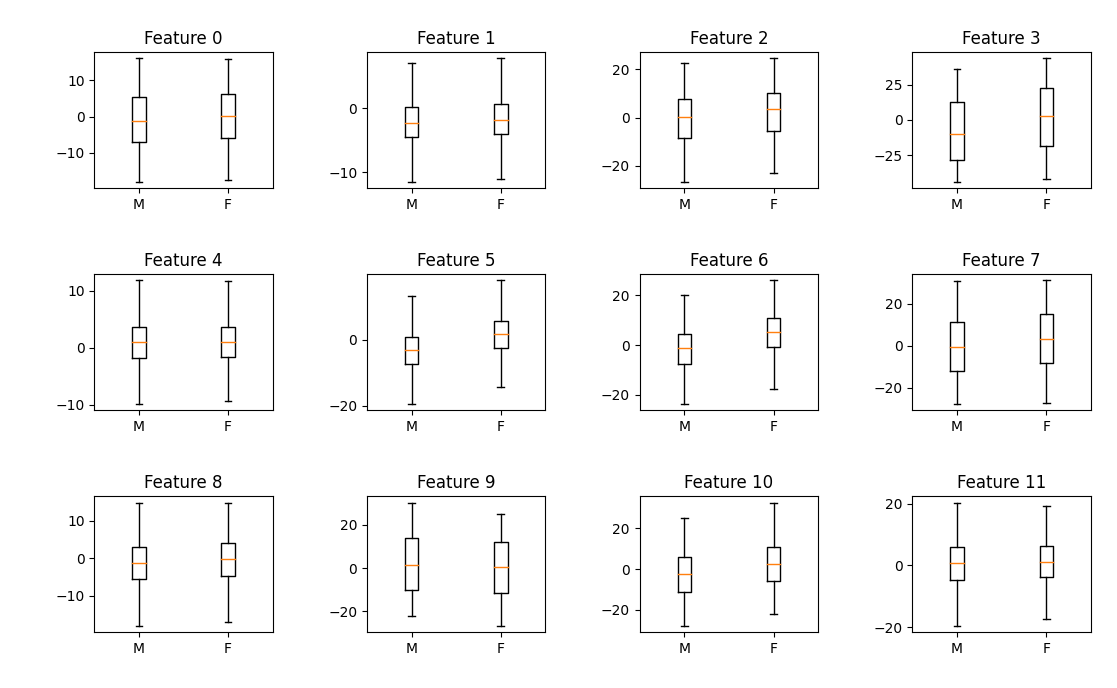
\includegraphics[width=\linewidth]{./Pictures/FeaturesAnalysis/boxplot.png}
	\caption{Raw features boxplots}
	\label{boxplot} 
\end{figure}

\subsection{Features distribution}
By plotting one histogram for each feature, separated for classes male and female, it is possible to show
if the samples (separately for each feature) follow a Gaussian distribution and how well. This
is done in order to understend whether a pre processing step like Gaussianization can be useful or not for our training data.
\begin{figure}[ht!]
	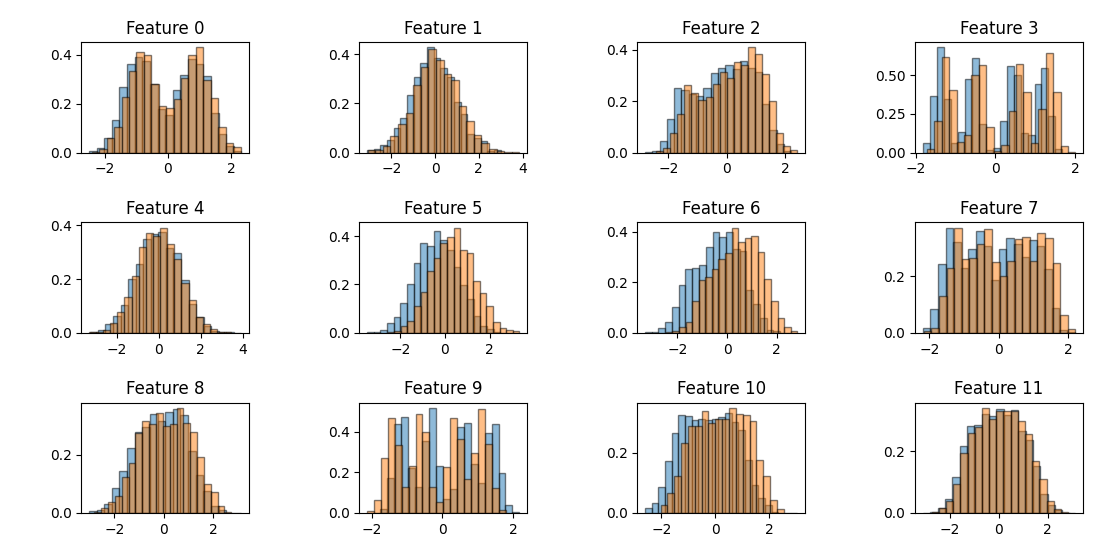
\includegraphics[width=\linewidth]{./Pictures/FeaturesAnalysis/hist_znorm.png}
	\caption{Z-normalized features distribution}
	\label{hist_znorm} 
\end{figure}

We can notice from figure \ref{hist_znorm} that almost all the features are already 
well-distributed (w.r.t. the Gaussian distribution) except for features 3, 7, 9. 
We can thus apply an additional pre-processing step in order to make all the features following a Gaussian distribution:
this step is called Gaussianization and it will be always applied after Z-Normalization preproccesing.

\subsubsection{Gaussianization}
Gaussianization is a pre-processing step that maps each fature to values whose empirical cumulative
distribution are well approximated by a Gaussian cumulative distribution function. For each
feature $x$ that we want to gaussianize we firstly compute the rank over the dataset:\\
\begin{center}
	\begin{math}
		r(x) = \frac{\sum_{i=1}^{N}\mathbb{I}[x_{i} < x] + 1}{N + 2}
	\end{math}
\end{center}
where $\mathbb{I}$ is the indicator function ($1$ when the condition inside $[\;]$ is true, $0$ 
otherwise). Actually, we are counting how many samples in the dataset $D$ have a greater value
with respect to the feature we are computing the rank on. \\
The next step is to compute the transformed feature as $y = \Phi^{-1}(r(x))$ where $\Phi$ is
the inverse of the cumulative distribution function. 

\begin{figure}[ht!]
	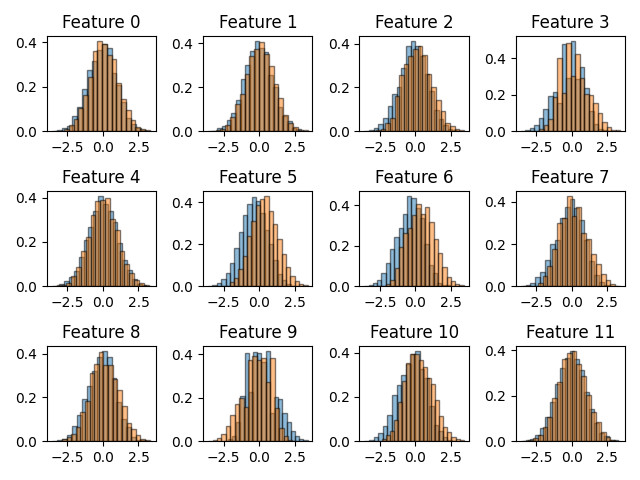
\includegraphics[width=\linewidth]{./Pictures/FeaturesAnalysis/hist_gau.png}
	\caption{Gaussianized features distribution}
	\label{hist_gau} 
\end{figure}
%%%%%%%%%%%%%%%
%%% HEATMAP %%%
%%%%%%%%%%%%%%%
\subsection{Features correlation}
We can show how much features are correlated by using a heatmap plot showing a darker
color inside cells $[i, j]$ for which it exists an high correlation among feaure $i$ and 
feature $j$. We are going to use the Pearson correlation coefficient to compute the
correlation among feature $X$ and feature $Y$:
\begin{center}
	\begin{math}
		|\frac{Cov(X, Y)}{\sqrt{Var(X)}\sqrt{Var(Y)}}|
	\end{math}
\end{center}
\begin{figure}[ht!]
	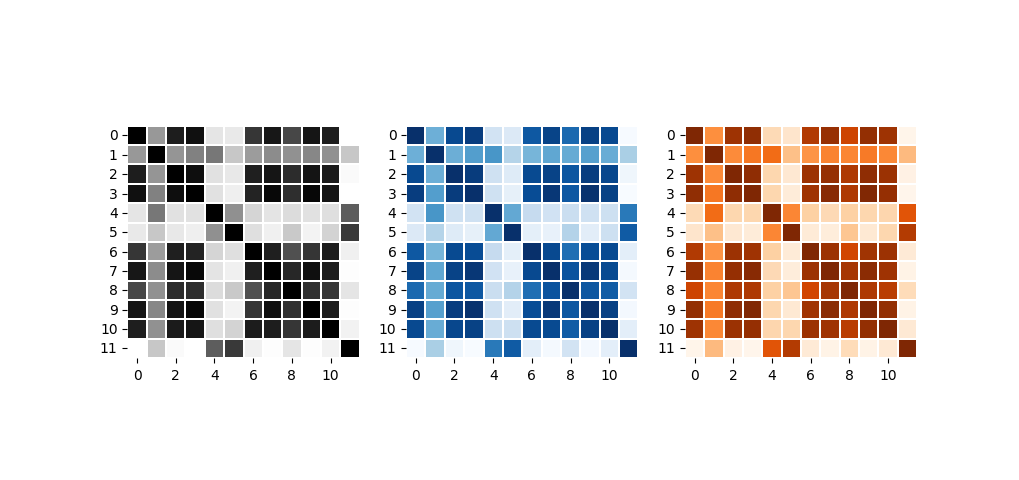
\includegraphics[width=\linewidth]{./Pictures/FeaturesAnalysis/heatmap_znorm.png}
	\caption{Z-normalized features correlation: grey the whole dataset, orange F class, 
	blue M class}
	\label{heatmap} 
\end{figure}

Correlation is quite high among most of the features. We can understand that applying PCA
would be meaningful for values of $m$ not below $11$ or $10$ at most. For smaller values of $m$
we would probably loose important information coming from high-correlated features. 
%%%%%%%%%%%%%%%%%%%%%%%%%%%%%%%%%%%%%%%%%%%
%%% DIMENSIONALITY REDUCTION DISCUSSION %%%
%%%%%%%%%%%%%%%%%%%%%%%%%%%%%%%%%%%%%%%%%%%
\section{Dimensionality reduction}
Before proceeding with the classification task we will spend some words on the possible 
dimensioanlity reduction rechniques that we have analyzed and that could be applied: PCA and LDA.
%%%%%%%%%%%%%%%%%%%%%%
%%% PCA DISCUSSION %%%
%%%%%%%%%%%%%%%%%%%%%%
\subsection{PCA}
As already anticipated, given the heatmap in figure \ref{heatmap} we can observe that PCA
with reasonable values of $m$ can be applied. 
PCA is a dimensionality reduction technique that, given a centered dataset $X = \{x_{1}, ..., x_{k}\}$, it aims to find the subspace of 
$\mathbb{R}^{n}$ that allows to preserve most of the information (the directions with the
highest variance).\\Starting from the sample covariance matrix
\begin{center}
	\begin{math}
		C = \frac{1}{K} \sum_{i}^{}(x_{i} - \bar{x})(x_{i}-\bar{x})^T
	\end{math}
\end{center}
we compute the eigen-decomposition of $C = U\Sigma U^T$ and project the data in the subspace
spanned by the $m$ columns of $U$ corresponding to the $m$ highest eigenvalues:
\begin{center}
	\begin{math}
		y_{i} = P^T(x_{i}-\bar{x})
	\end{math}
\end{center}
where $P$ is the matrix corresponding the the $m$ columns of $U$ associated the to
the $m$ highest eigenvalues of $C$.
In this preliminary analysis, in order to select the optimal $m$, we can use a cross-validation approach by inspecting how much
of the total variance of the data we are able to retain by using different values for $m$. We exploit the fact
that each eigenvalue corresponds to the variance along the corresponding axis and the
eigenvalues are the elements of the diagonal of the matrix $\Sigma$. We selecte $m$ as:
\begin{center}
	\begin{math}
		\min_m\;s.t \frac{\sum_{i}^{m}\sigma_{i}}{\sum_{i}^{n}\sigma_{i}} \ge t
	\end{math}
\end{center}
\begin{figure}[ht!]
	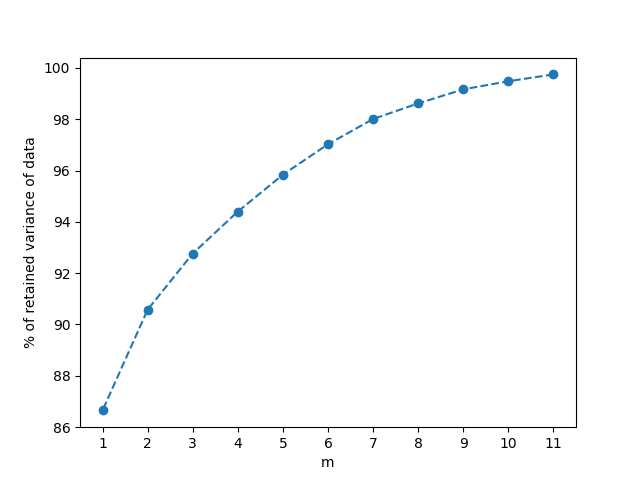
\includegraphics[width=\linewidth]{./Pictures/FeaturesAnalysis/pca.png}
	\caption{3-fold cross validation for PCA impact evaluation}
	\label{pca} 
\end{figure}
We can clearly understand from figure \ref{pca} that values of $m < 9$ would rapidly
decrease the amout of retained variance of the data. We will see better later on how 
choosing a too small value of $m$ would badly impact the performances of the different classifiers.

%%%%%%%%%%%%%%%%%%%%%%
%%% LDA DISCUSSION %%%
%%%%%%%%%%%%%%%%%%%%%%
\subsection{LDA}
PCA technique is unsupervised so we have no guarantee of obtainig discriminant directions.
Despite the fact that LDA allows to find at most $C - 1$ discriminant directions (where $C$ is the number of classes), so 
it makes no sense to apply it as a dimensionality reduction technique in a bianry classification task, it can
be used as a linear classifier and we can understand it by its definition; LDA mazimizes the
between-class variability over the within-class variability ratio for the transformed samples:
\begin{center}
	\begin{math}
		\mathcal{L}(w) = \frac{s_{B}}{s_{W}} = \max_w \frac{w^TS_{B}w}{w^TS_{W}w}
	\end{math}
\end{center}
It can be proved that the optimal solution corresponds to the eigenvector of $S_{W}^-1S_{B}$ 
corresponding to the largest eigenvalue. Once that we have estimated $w$ we can project
the test samples over $w$ and assign the class label looking at the score obtained:\\
\begin{center}
	\begin{math}
		C(x_t)=\left\{
		\begin{array}{ll}
			C_1, & \mbox{if $w^Tx_t \ge t$}.\\
			C_0, & \mbox{if $w^Tx_t < t$}.
		\end{array}
		\right.
	\end{math}
\end{center}
It will be proved later how this model
is related to the Tied Gaussian Generative Classifier model.
\section{Classification models analysis}
%%%%%%%%%%%%%%%%%%%%%%%%%%%%
%%% CLASSIFICATION INTRO %%%
%%%%%%%%%%%%%%%%%%%%%%%%%%%%
\subsection{Premises}
In the next paragraphs we are going to compare different classification models. 
We will employ a k-fold cross validation technique (with $k=3$) for model evaluation.
We will consider three types of applications:
\begin{center}
	$(\tilde{\pi}, C_{fp}, C_{fn}) = (0.1, 1, 1)$\\
	$(\tilde{\pi}, C_{fp}, C_{fn}) = (0.5, 1, 1)$\\
	$(\tilde{\pi}, C_{fp}, C_{fn}) = (0.9, 1, 1)$\\
\end{center}
and the target application (the one we will optimize for) will be the balanced one:
\begin{center}
	$(\tilde{\pi}, C_{fp}, C_{fn}) = (0.5, 1, 1)$
\end{center}
We are interested
in selecting the most promising approach and we will infact perform measures in term of minimum
detection cost:
\begin{center}
	\begin{math}
		DCF = \frac{DCF_{u}(\pi_{T}, C_{fn}, C_{fp})}{min(\pi_{T},C_{fn}, (1-\pi_{T}C_{fp}))} = 
			\frac{\pi_{T}C_{fn}P_{fn} + (1-\pi_{T})C_{fp}P_{fp}}{min(\pi_{T},C_{fn}, (1-\pi_{T}C_{fp}))}
	\end{math}
\end{center}
and for $minDCF$ computation we will look for the threshold:
\begin{center}
	\begin{math}
		t' = -log(\frac{\tilde{\pi}}{1-\tilde{\pi}})
	\end{math}
\end{center}
that allows us to obtain the lowest possible $DCF$ (as if we knew in advance this optimal value fot threshold).
%%%%%%%%%%%%%%%%%%%%%%%
%%% GAUSSIAN MODELS %%%
%%%%%%%%%%%%%%%%%%%%%%%
\subsection{Gaussian models}
The first class of models we are going to analyze are the generative Gaussian models. We assume that,
given the dataset $X$, the sample $x_{t}$ is a realization of the R.V. $X_{t}$. A simple
model consists in assuming that our data, given the class, can be described by a Gaussian distribution:
\begin{center}
	\begin{math}
		(X_{t}|C_{t}=c) \sim (X|C=c) \sim \mathcal{N} (x_{t}|\mu_{c},\Sigma_{c})
	\end{math}
\end{center}
Since we are dealing with a binary classification task 
we will assign a probabilistic score to each sample in terms of the class-posterior 
log-likelihood ratio:
\begin{center}
	\begin{math}
		llr(x_t)=log\;r(x_{t}) = log\;\frac{P(C = h_{1}|x_{t})}{P(C = h_{0}|x_{t})}
	\end{math}
\end{center}
We can expand this expression by writing:
\begin{center}
	$log\;r(x_{t}) = log\;\frac{f_{X|C}(x_{t}|h_{1})}{f_{X|C}(x_{t}|h_{0})} + log\;\frac{\pi}{1-\pi}$
\end{center}
\begin{center}
	with\;$ f_{X|C}(x_{t}|c) = \mathcal{N}(x|\mu_c,\Sigma_c)$
\end{center}
While the training phase consists in estimating the model parameters of the Mutlivariate Gaussian
distribution the scoring phase
consists in computing the log-likelihood ratio (first term of the equation) for each sample. 
It will be then compared with  a threshold specific for each application to compute
the $minDCF$. What it differentiates the different Gaussian models is the way how we estimate the
model parameters of the Gaussian distribution.

\subsubsection{MVG Gaussian Classifier}
The ML solution to the previous described problem is given by the empirical mean and covariance
matrix for each class:
\begin{center}
	$\mu_{c}^* = \frac{1}{N_c}\sum_{i=1}^{N}x_{c,i}$ \\
	$\Sigma_c^* = \frac{1}{N_c}\sum_{i=1}^{N}(x_{c,i}-\mu_c^*)(x_{c,i}-\mu_c^*)^T$
\end{center}
\subsubsection{Naive Bayes Classifier}
The Naive Bayes assumption simplifies the MVG full covariance model stating that if we knew
that for each class the components are approximately independent we can assume that the 
distribution $X|C$ can be factorized over its components. The ML solution to this problem is:
\begin{center}
	$\mu_{c,[j]}^* = \frac{1}{N_c}\sum_{i|c_i=c}^{}x_{i,[j]}$ \\
	$\sigma_{c,[j]}^2 = \frac{1}{N_c}\sum_{i|c_i=c}^{}(x_{i,[j]}-\mu_{c,[j]})^2$
\end{center}
The density of a sample $x$ can be expressed as $\mathcal{N}(x|\mu_c,\Sigma_c)$ where
$\mu_c$ is an array where each element $\mu_{c,[j]}$ is the the mean for each class
for each component while $\Sigma_c$ is a diagonal covariance matrix. The Naive Bayes classifier
corresponds to the MVG full covariance classifier with a diagonal covariance matrix.
\subsubsection{Tied Gaussian Classifier}
This model assumes that the covariance matrices of the different classes are tied (we consider
only one covariance matrix common to all classes). We are assuming that:
\begin{center}
	$f_{X|C}(x|c) = \mathcal{N} (x|\mu_c, \Sigma)$
\end{center}
so each class has its own mean but the covariance matrix is the same for all the classes. The ML
solution to this problem is:
\begin{center}
	$\mu_{c}^* = \frac{1}{N_c}\sum_{i=1}^{N}x_{c,i}$ \\
	$\Sigma^* = \frac{1}{N}\sum_c{}^{}\sum_{i|c_i=c}^{}(x_{i}-\mu_c^*)(x_{i}-\mu_c^*)^T$
\end{center}
This model is strongly related to LDA (used as a linear classfication model). By considering 
the binary log-likelihood ratio of the tied model we obtain a linear decision function:
\begin{center}
	$llr(x) = log\;\frac{f_{X|C}(x|h_1)}{f_{X|C}(x|h_0)} = x^Tb + c$ 
\end{center}
where $b$ and $c$ are functions of class means and (tied) covariance matrix. On the other hand,
projecting over the LDA subspace is, up to a scaling factor $k$, given by:
\begin{center}
	$w^Tx = k \cdot x^T\varLambda (\mu_1-\mu_0)$ 
\end{center}
where $\varLambda (\mu_1-\mu_0) = b$. The LDA assumption that all the classes have the same
within class covariance matrix is related to the assumption done for the tied model.\\
\subsubsection{Gaussian Models Comparison}
\FloatBarrier
	\begin{table}
		\caption{Gaussian Models}
		\centering
		\begin{tabular}{ |l|l|l|l| }
			\hline
			& $\tilde{\pi}=0.1$ & $\tilde{\pi}=0.5$ & $\tilde{\pi}=0.9$ \\ \hline
			\multicolumn{4}{ |c| }{\bf{Z-normalized features - no PCA}} \\
			\hline
			\multirow{3}{*}{}
			 Full Cov & 0.128 & 0.048 & 0.125\\
			 Tied Cov & 0.122 & \textcolor{red}{0.046} & 0.127\\
			 Naive Bayes & 0.822 & 0.567 & \textcolor{blue}{0.856}\\
			\hline
			\multicolumn{4}{ |c| }{\bf{Z-normalized features - PCA(m=11)}} \\
			\hline
			\multirow{3}{*}{}
			 Full Cov & 0.265 & 0.100 & 0.231\\
			 Tied Cov & 0.257 & \textcolor{red}{0.098} & 0.227\\
			 Naive Bayes & \textcolor{orange}{0.278} & \textcolor{orange}{0.108} & \textcolor{orange}{0.245}\\
			\hline
			\multicolumn{4}{ |c| }{\bf{Z-normalized features - PCA(m=10)}} \\
			\hline
			\multirow{3}{*}{}
			 Full Cov & 0.303 & 0.115 & 0.267\\
			 Tied Cov & 0.293 & \textcolor{red}{0.112} & 0.264\\
			 Naive Bayes & \textcolor{orange}{0.306} & \textcolor{orange}{0.121} & \textcolor{orange}{0.283}\\
			\hline
			\multicolumn{4}{ |c| }{\bf{Gaussianized features - no PCA}} \\
			\hline
			\multirow{3}{*}{}
			 Full Cov & 0.218 & \textcolor{red}{0.078} & 0.191\\
			 Tied Cov & 0.208 & \textcolor{red}{0.078} & 0.189\\
			 Naive Bayes & 0.813 & 0.586 & \textcolor{blue}{0.847} \\
			\hline
			\multicolumn{4}{ |c| }{\bf{Gaussianized features - PCA(m=11)}} \\
			\hline
			\multirow{3}{*}{}
			 Full Cov & 0.227 & 0.087 & 0.218\\
			 Tied Cov & 0.215 & \textcolor{red}{0.084} & 0.208\\
			 Naive Bayes & \textcolor{blue}{0.278} & \textcolor{orange}{0.106} & 0.257\\
			\hline
			\multicolumn{4}{ |c| }{\bf{Gaussianized features - PCA(m=10)}} \\
			\hline
			\multirow{3}{*}{}
			 Full Cov & 0.223 & 0.084 & 0.211\\
			 Tied Cov & 0.212 & \textcolor{red}{0.082} & 0.207\\
			 Naive Bayes & \textcolor{blue}{0.279} & \textcolor{orange}{0.103} & 0.254\\
			\hline
		\end{tabular}
	\end{table}
\FloatBarrier

A graphical version of the table can be helpful in analyzing results:
\begin{figure}[ht!]
	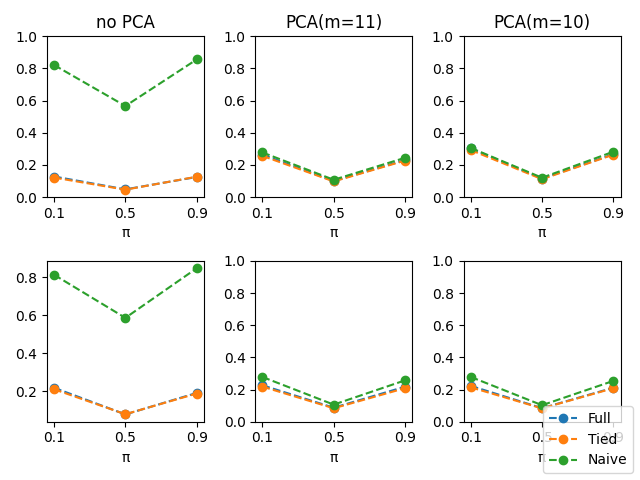
\includegraphics[width=\linewidth]{./Pictures/FeaturesAnalysis/gaumodels.png}
	\caption{Top: Z-Normalized feautres, Bottom: Gaussianized features}
	\label{gauplots} 
\end{figure}

\begin{itemize}
	\item We can notice that Full-Cov model and Tied-Cov model achieve very good and similar results with
		  slighlty better performances for the Tied-Cov model (this means that the covariance matrices
		  of the different classes are similar and infact the model provides more robust estimates
		  in this case).
	\item Gaussianization pre processing does't really help in achieving better results because 
	      data are already well distributed according to the Gaussian assumptions (this was also noticed
		  previously while discussing the Gaussianization pre-processing).
	\item Naive Bayes assumption doesn't hold really well, in particular if PCA is not applied. When 
		  PCA is applied it has a really good impact only on Naive Bayes model and especialliy if also
		  combined with Gaussianization pre-processing (the Naive Bayes assumption that the covariance
		  matrix of each class is diagonal holds better with lower features dimensionality and improved
		  features distribution from a Gaussian point of view).
	\item Regarding Full and Tied models with PCA(m=11) there is no a high performance degradation
		  since the minDCFs values obtained are still good. For lower values of $m$ the models become less
		  able in taking decisions and the minDCF increases
	\item For the MVG classifiers best performances are achieved by the Tied-Cov classifier with
		  only Z-normalization pre processing and withouth PCA. Really good performacnes are also
		  achieved by the Tied-Cov model trained with Gaussianized
		  fetures and no-PCA (the PCA(m=11) version of this model achieves worse but comparable result w.r.t. to the no-PCA version
		  and it can be selected to try to better avoid overfitting by reducing the features 
		  space and also for reducing computational effort)
\end{itemize}
\underline{Best Gaussian Models}: 
\begin{itemize}
	\item Tied Cov (Z-Normalization, no PCA)
	\item Tied Cov (Gaussianization, PCA(m=11))
\end{itemize}
%%%%%%%%%%%%%%%%%%%%%%%%%%%%%%%%%%%%%%%%%%%%%%%%%%%%%%%%%%%%
%%%%%%%%%%%%%%%%%%%%%% LOGREG CLASSIFIER %%%%%%%%%%%%%%%%%%%
%%%%%%%%%%%%%%%%%%%%%%%%%%%%%%%%%%%%%%%%%%%%%%%%%%%%%%%%%%%%
\subsection{Logistic Regression Classifier}
Logistic Regression is a discriminative classification model. Starting from the results obtained
from the Tied Gaussian classifier we consider the linear decision function obtained from the expression
of the posterior log-likelihood ratio:
\begin{center}
	\begin{math}
		l(x) = log\;\frac{P(C=h_1|x)}{P(C=h_0|x)}=log\;\frac{f_{X|C}(x|h_1)}{f_{X|C}(x|h_0)} + log\;\frac{\pi}{1-\pi} = w^Tx + b
	\end{math}
\end{center}
where $b$ takes into account all the prior information. Given $w$ and $b$ we can compute the
expression for the posterior class probability:
\begin{center}
	\begin{math}
		P(C=h_1|x,w,b)=\frac{e^{(w^Tx + b)}}{1+e^{(w^Tx+b)}}=\sigma(w^Tx+b)
	\end{math}
\end{center}
where $\sigma(x)=\frac{1}{1+e^{-x}}$ is the sigmoid function. LR assumes that the decision rules will be hyperplanes
orthogonal to $w$.
\subsubsection{Linear Logistic Regression (LLR)}
We are going to look for the minimizer of the function:
\begin{center}
	\begin{math}
		J(w,b) = \frac{\lambda}{2}||w||^2 + \frac{1}{n}\sum_{i=1}^{n}log(1 + e^{-z_i(w^Tx_i+b)})
	\end{math}
\end{center}
where $\lambda$ is an hyperparameter that represents the regularization term (needed to make the 
problem solvable in case of linearly separable classes).
\begin{figure}[ht!]
	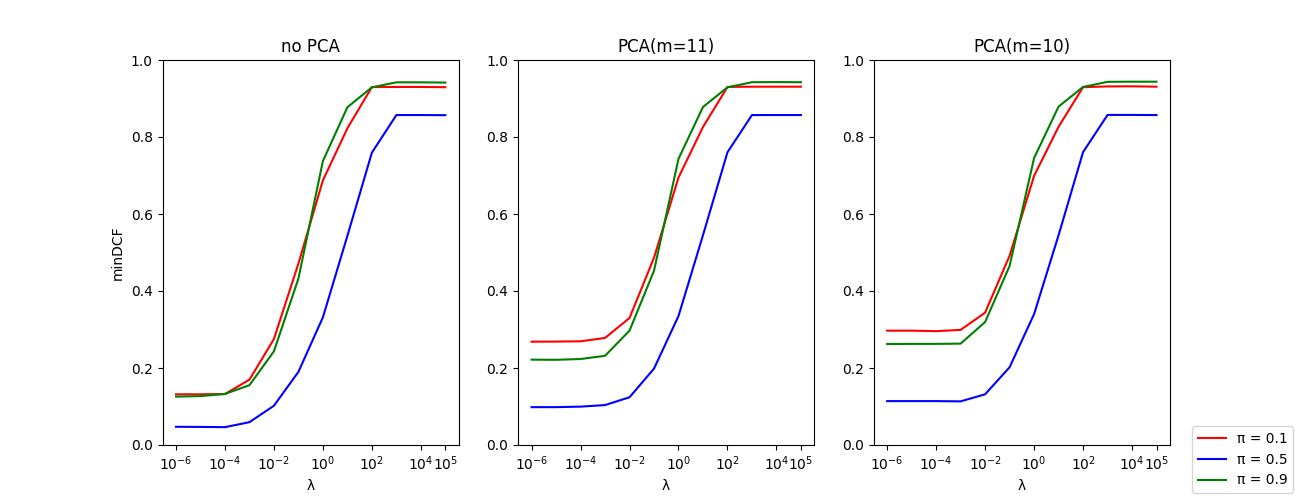
\includegraphics[width=\linewidth]{./Pictures/FeaturesAnalysis/dcfplotLLR.png}
	\caption{minDCF for different values of $\lambda$ and different priors}
	\label{dcfLLR} 
\end{figure}
\begin{table}[ht!]
		\caption{Linear Logistic Regression - 3-fold cross validation}
		\centering
		\begin{tabular}{ |l|l|l|l| }
			\hline
			& $\tilde{\pi}=0.1$ & $\tilde{\pi}=0.5$ & $\tilde{\pi}=0.9$ \\ \hline
			\multicolumn{4}{ |c| }{\bf{Z-normalized features - no PCA}} \\
			\hline
			\multirow{3}{*}{}
			 LLR \scriptsize{($\lambda=10^{-3}$)}& \textcolor{blue}{0.170} & 0.059 & 0.155\\
			 LLR \scriptsize{($\lambda=10^{-5}$)}& 0.132 & \textcolor{red}{0.047} & 0.127\\
			 LLR \scriptsize{($\lambda=10^{-6}$)}& 0.132 & \textcolor{red}{0.047} & 0.126\\
			\hline
			\multicolumn{4}{ |c| }{\bf{Z-normalized features - PCA(m=11)}} \\
			\hline
			\multirow{3}{*}{}
			 LLR \scriptsize{($\lambda=10^{-3}$)}& \textcolor{blue}{0.278} & 0.104 & 0.232\\
			 LLR \scriptsize{($\lambda=10^{-5}$)}& 0.269 & \textcolor{red}{0.098} & 0.221\\
			 LLR \scriptsize{($\lambda=10^{-6}$)}& 0.268 & 0.098 & 0.222\\
			 \hline
			 \multicolumn{4}{ |c| }{\bf{Z-normalized features - PCA(m=10)}} \\
			 \hline
			 \multirow{3}{*}{}
			  LLR \scriptsize{($\lambda=10^{-3}$)}& \textcolor{blue}{0.299} & \textcolor{red}{0.113} & 0.263\\
			  LLR \scriptsize{($\lambda=10^{-5}$)}& 0.297 & 0.114 & 0.263\\
			  LLR \scriptsize{($\lambda=10^{-6}$)}& 0.297 & 0.114 & 0.262\\
			 \hline
		\end{tabular}
	\end{table}
\begin{table}[ht!]
		\caption{Best models analyzed up to now}
		\centering
		\begin{tabular}{ |l|l|l|l| }
			\hline
			& $\tilde{\pi}=0.1$ & $\tilde{\pi}=0.5$ & $\tilde{\pi}=0.9$ \\ \hline
			\multicolumn{4}{ |c| }{\bf{Gaussian Models}} \\
			\hline
			\multirow{2}{*}{}
			 Tied Cov \scriptsize{(Z-Norm, no PCA)}& 0.122 & 0.046 & 0.127\\
			 Tied Cov \scriptsize{(Gau, PCA(m=10))}& 0.212 & 0.082 & 0.207\\
			\hline
		\end{tabular}
\end{table}
\begin{itemize}
	\item The choice of $\lambda$ appear to be critical for all the applications, in particular for the 
	unbalanced ones. By observing figure \ref{dcfLLR} it is clear that for values of $\lambda$ greater
	than $10^{-3}$ the $minDCF$ rapidly increases for all the considered applications.
	\item PCA never helps in achieving better results.
\end{itemize}
\textit{Comparison}: the LLR model trained with $\lambda=10^{-6}$ and no-PCA achieves really similar results
with the ones achieved by the Tied-Cov Gaussian model (Z-Norm, no PCA) for $\tilde{\pi}=0.5$ and $\tilde{\pi}=0.9$
applications but a worse performance is obtained for $\tilde{\pi}=0.1$. The LLR model behaves better than the
Tied-Cov Gaussian model (Gau, PCA(m=10)) in all the three applications.\\
\underline{Selected LLR Model}: 
\begin{itemize}
	\item Z-normalized features, $\lambda=10^{-6}$, no PCA
\end{itemize}
\subsubsection{Quadratic Logistic Regression (QLR)}
Now we are going to train a Quadratic LR model by performing features expansion.
For binary linear LR the separation surfaces are linear decision functions as already discussed (and
we obtain the same form as for the Tied Gaussian classifier). By looking instead at the separation surface
obtained through the MVG Gaussian classifier we have:
\begin{center}
	\begin{math}
		log\;\frac{P(C=h_1|x)}{P(C=h_0|x)} = x^TAx + b^Tx + c = s(x, A, b, c)
	\end{math}
\end{center}
This expression is quadratic in $x$ but it's linear in $A$ and $b$. 
We could rewrite it to obtain a decision function that is linear for the expanded features space
but quadratic in the original features space. Features expansion is defined as:
\begin{center}
	\begin{math}
		\Phi(x) = \begin{bmatrix}
					vec(xx^T)\\
					x
				  \end{bmatrix} \;, 
		w= 		 \begin{bmatrix}
					vec(A)\\
					b
				  \end{bmatrix}
	\end{math}
\end{center}
where $vec(X)$ is the operator that stacks the columns of $X$. In this way the posterior log-likelihood is expressed as:
\begin{center}
	\begin{math}
		s(x, w, c) = s^T\phi(x)+c
	\end{math}
\end{center}
We are now going to train the Linear Logistic Regression model using features vectors $\phi(x)$.\\
\begin{figure}[ht!]
	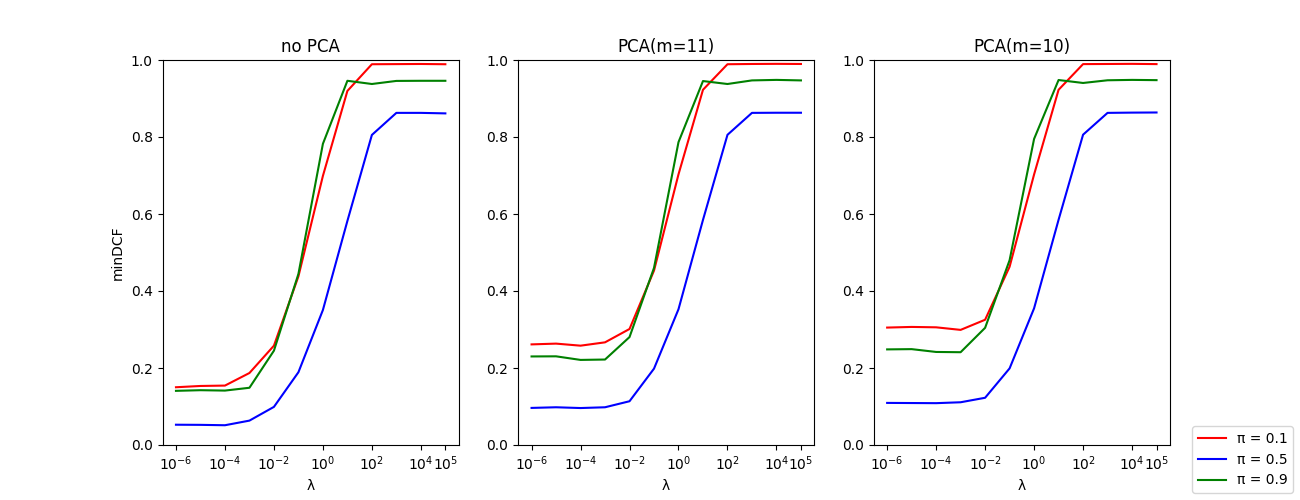
\includegraphics[width=\linewidth]{./Pictures/FeaturesAnalysis/dcfplotQLR.png}
	\caption{minDCF for different values of $\lambda$ and different priors}
	\label{dcfQLR} 
\end{figure}
\begin{table}[ht!]
	\caption{Quadratic Logistic Regression - 3-fold cross validation}
	\centering
	\begin{tabular}{ |l|l|l|l| }
		\hline
		& $\tilde{\pi}=0.1$ & $\tilde{\pi}=0.5$ & $\tilde{\pi}=0.9$ \\ \hline
		\multicolumn{4}{ |c| }{\bf{Z-normalized features - no PCA}} \\
		\hline
		\multirow{3}{*}{}
		 QLR \scriptsize{($\lambda=10^{-3}$)}& \textcolor{blue}{0.187} & 0.063 & 0.149\\
		 QLR \scriptsize{($\lambda=10^{-5}$)}& 0.153 & \textcolor{red}{0.052} & 0.142\\
		 QLR \scriptsize{($\lambda=10^{-6}$)}& 0.150 & 0.053 & 0.141\\
		\hline
		\multicolumn{4}{ |c| }{\bf{Z-normalized features - PCA(m=11)}} \\
		\hline
		\multirow{3}{*}{}
		 QLR \scriptsize{($\lambda=10^{-3}$)}& 0.267 & 0.098 & \textcolor{orange}{0.222}\\
		 QLR \scriptsize{($\lambda=10^{-5}$)}& \textcolor{orange}{0.263} & 0.098 & 0.230\\
		 QLR \scriptsize{($\lambda=10^{-6}$)}& 0.305 & \textcolor{red}{0.096} & 0.230\\
		\hline
		\multicolumn{4}{ |c| }{\bf{Z-normalized features - PCA(m=10)}} \\
		\hline
		\multirow{3}{*}{}
		 QLR \scriptsize{($\lambda=10^{-3}$)}& 0.299 & 0.111 & 0.241\\
		 QLR \scriptsize{($\lambda=10^{-5}$)}& \textcolor{blue}{0.307} & \textcolor{red}{0.109} & 0.249\\
		 QLR \scriptsize{($\lambda=10^{-6}$)}& 0.305 & 0.109 & 0.248\\
		\hline
	\end{tabular}
\end{table}
\begin{table}[ht!]
	\caption{Best models analyzed up to now}
	\centering
	\begin{tabular}{ |l|l|l|l| }
		\hline
		& $\tilde{\pi}=0.1$ & $\tilde{\pi}=0.5$ & $\tilde{\pi}=0.9$ \\ \hline
		\multicolumn{4}{ |c| }{\bf{Gaussian Models}} \\
		\hline
		\multirow{2}{*}{}
		 Tied Cov \scriptsize{(Z-Norm, no PCA)}& 0.122 & 0.046 & 0.127\\
		 Tied Cov \scriptsize{(Gau, PCA(m=10))}& 0.212 & 0.082 & 0.207\\
		\hline
		\multicolumn{4}{ |c| }{\bf{Logistic Regression Models}} \\
		\hline
		\multirow{1}{*}{}
		LLR &&&\\\scriptsize{(Z-Norm, $\lambda=10^{-6}$, no PCA)}& 0.132 & 0.047 & 0.126\\
		\hline
	\end{tabular}
\end{table}

\begin{itemize}
	\item By rapidly looking at the results obtained we can say that quadratic version of the logistic regression
	performs worse w.r.t the linear version (the one without features expansion).
	\item The choice of $\lambda$ is still critical and $\lambda <= 10^{-5}$ still remains the best choice
	\item Regarding the target application
	we are able to reach similar results comparing to the linear version of the LR while the unbalanced applications
	are more penalized.
	\item When PCA is applied no effective improvements are obtained.
	
\end{itemize}


\textit{Comparison}: With respect to Gaussian models comparable performances are achieved for $\lambda=10^{-6}$ and
no PCA even if the model performs slightly worse. The quadratic model performs also worse than the linear model and
we won't consider it in score calibration.
\\ 
\underline{Selected QLR Model}: 
\begin{itemize}
	\item Z-Normalized features, $\lambda=10^{-5}$, no PCA
\end{itemize}
%%%%%%%%%%%%%%%%%%%%%%%%%%%%%%%%%%%%%%%%%%%%%%%%%%%%%%%%%%%%
%%%%%%%%%%%%%%%%%%%%%% SVM CLASSIFIER %%%%%%%%%%%%%%%%%%%%%%
%%%%%%%%%%%%%%%%%%%%%%%%%%%%%%%%%%%%%%%%%%%%%%%%%%%%%%%%%%%%
\subsection{SVM Classifier}
% ---- LINEAR SVM MATH ----
\subsubsection{Linear SVM}
Support Vector Machines are linear classifiers that look for maximum margin separation hyperplanes.
The primal formulation of the soft-margin SVM problem consists in minimizing the function:
\begin{center}
	\begin{math}
		J(w,b)=\frac{1}{2}||w^2|| + C\sum_{i=1}^{N}max(0, 1-z_i(w^Tx_i+b))
	\end{math}
\end{center}
where $N$ is the number of trainig samples and $C$ is an hyperparameter.\\
We are also going to take into account the dual formulation to solve the problem that consists in maximizing the function:
\begin{center}
	\begin{math}
		J^D(\alpha)=-\frac{1}{2}\alpha^TH\alpha + \alpha^T\textbf{1} \; s.t.\; 0 \le \alpha_i \le C \;and\;\sum_{i=1}^{n}\alpha_iz_i=0 \; \forall i\in \{1,...,n\}
	\end{math}
\end{center}
where $\textbf{1}$ is a $n$-dimensional vector of ones and $H$ is the matrix
whose elements are $H_{ij} = z_iz_jx_i^Tx_j$.\\
From the constraints of the Lagrangian problem that allows to introduce the dual formulation
we can obtain that:
\begin{center}
	$w^*=\sum_{i=1}^{n}\alpha_i^*z_ix_i$
\end{center}
and the optimal bias $b$ can be computed considering a sample $x_i$ that lies on the margin: $z_i(w^{*T}x_i+b^*)=1$.
To be able to computationally solve the problem
we need to modify the primal formulation as:
\begin{center}
	\begin{math}
		\hat{J}(\hat{w})=\frac{1}{2}||\hat{w}||^2 + C\sum_{i=1}^{N}max(0, 1-z_i(\hat{w}^T\hat{x}_i))
	\end{math}
\end{center}
where $\hat{x}_i = \begin{bmatrix} x_i\\ 1 \end{bmatrix}$ and $\hat{w} = \begin{bmatrix} w\\ b \end{bmatrix}$.\\
The scoring rule $\hat{w}^T\hat{x}_i = w^Tx + b$ has the same form of the original formulation but
we are also regularizing the norm of $\hat{w}: ||\hat{w}||^2 = ||w||^2 + b^2$ and we use a mapping
$\hat{x}_i = \begin{bmatrix} x_i\\ K \end{bmatrix}$ to mitigate the fact that by regularizing  the bias
term we could obtain sub-optimal results. According to the modification done to
the primal formulation we also modify the dual formulation as:
\begin{center}
	\begin{math}
		J^D(\alpha)=-\frac{1}{2}\alpha^T\hat{H}\alpha + \alpha^T\textbf{1} \; s.t.\; 0 \le \alpha_i \le C, \forall i\in \{1,...,n\}
	\end{math}
\end{center}
where the equality constraint dissapeared (the one that L-BFGS was not able to incorporate) and the
matrix $\hat{H}$ can be computed as $\hat{H}_{i,j}=z_iz_j\hat{x}_i^T\hat{x}_j$
% ---- LINEAR SVM MINDCF PLOT ----
\begin{figure}[ht!]
	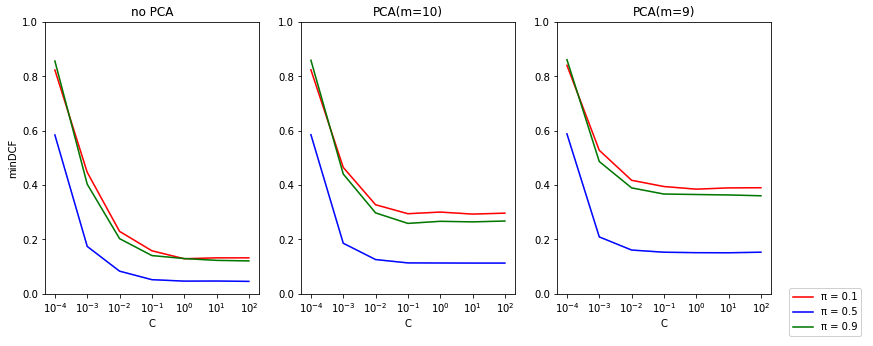
\includegraphics[width=\linewidth]{./Pictures/FeaturesAnalysis/LSVM.png}
	\caption{Linear SVM (K=0, Z-Normalized features) - minDCF for different values of $C$ and different priors}
	\label{lsvm} 
\end{figure}
% ---- LINEAR SVM TABLE ----
\begin{table}[ht!]
	\caption{Linear SVM - 3-fold cross validation}
	\centering
	\begin{tabular}{ |l|l|l|l| }
		\hline
		& $\tilde{\pi}=0.1$ & $\tilde{\pi}=0.5$ & $\tilde{\pi}=0.9$ \\ \hline
		\multicolumn{4}{ |c| }{\bf{Z-normalized features - no PCA}} \\
		\hline
		\multirow{2}{*}{}
		 Linear SVM \scriptsize{($C=0.1$)}& \textcolor{blue}{0.158} & 0.052 & 0.141\\
		 Linear SVM \scriptsize{($C=1$)}& 0.129 & \textcolor{red}{0.047} & 0.130\\
		\hline
		\multicolumn{4}{ |c| }{\bf{Z-normalized features - PCA(m=11)}} \\
		\hline
		\multirow{2}{*}{}
		Linear SVM \scriptsize{($C=0.1$)}& \textcolor{blue}{0.275} & 0.102 & 0.233\\
		Linear SVM \scriptsize{($C=1$)}& 0.269 & \textcolor{red}{0.100} & 0.226\\
		\hline
		\multicolumn{4}{ |c| }{\bf{Z-normalized features - PCA(m=10)}} \\
		\hline
		\multirow{2}{*}{}
		Linear SVM \scriptsize{($C=0.1$)}& 0.295 & 0.114 & 0.259\\
		Linear SVM \scriptsize{($C=1$)}& \textcolor{blue}{0.301} & \textcolor{red}{0.113} & 0.267\\
		\hline
	\end{tabular}
\end{table}
% ---- BEST MODELS ----
\begin{table}[ht!]
	\caption{Best models analyzed up to now}
	\centering
	\begin{tabular}{ |l|l|l|l| }
		\hline
		& $\tilde{\pi}=0.1$ & $\tilde{\pi}=0.5$ & $\tilde{\pi}=0.9$ \\ \hline
		\multicolumn{4}{ |c| }{\bf{Gaussian Models}} \\
		\hline
		\multirow{2}{*}{}
		 Tied Cov \scriptsize{(Z-Norm, no PCA)}& 0.122 & 0.046 & 0.127\\
		 \hline
		 Tied Cov \scriptsize{(Gau, PCA(m=10))}& 0.212 & 0.082 & 0.207\\
		\hline
		\multicolumn{4}{ |c| }{\bf{Logistic Regression Models}} \\
		\hline
		\multirow{2}{*}{}
		LLR &&&\\\scriptsize{(Z-Norm, $\lambda = 10^{-6}$, no PCA)}& 0.132 & 0.047 & 0.126\\
		\hline
		QLR &&&\\\scriptsize{(Z-Norm, $\lambda = 10^{-5}$, no PCA)}& 0.153 & 0.052 & 0.142\\
		\hline
	\end{tabular}
\end{table}
The only preprocessing step that has been considered is Z-normalization. As we can notice from figure \ref{lsvm}
better results are achieved for smaller values of the hyperparameter $C$ so the choice of it is crucial.
% ---- LINEAR SVM CONSIDERATIONS ---
\begin{itemize}
	\item Best performances on the target application are reached for $C=1$ combined with
		  Z-normalized features and no PCA.
	\item PCA is not helpful in reducing the minDCF in any of the considered applications
		  even if with PCA(m=11) there is no a high performance degradation for the target
		  application.
\end{itemize}
% ---- LINEAR SVM COMPARISON ---
\textit{Comparison}: The results achieved by the model trained with Z-normalization, 
$C=1$ and no PCA are closed to the the results obtained by the Linear Logistic Regression Model
but slighlty worse with respect to the results obtained by the Tied Gaussian model.
\underline{Selected Linear SVM Model}: \\Z-normalized features - K=0, C=1 - no PCA
% ---- KERNEL SVM MATH ----
\subsubsection{Kernel SVM}
SVMs allow for non-linear classification through an implicit expansion of the features in a higher
dimensional space. In contrast with Quadratic Logistic Regression classifier we don't have to compute
an explicit expansion of the features space, it is sufficient to be able to compute the scalar product between
the expanded features: $k(x_1, x_2) = \phi(x_1)^T\phi(x_2)$ where $k$ is the kernel function. We have to 
replace $\hat{H}$ with $\hat{H} = z_iz_jk(z_1,x_2)$. We are going to implement two types of kernel: polynomial and rbf.
\begin{itemize}
	\item Polynomial kernel of degree $d$: 
\end{itemize}
		\begin{center}
			$k(x_1, x_2) = (x_1^Tx_2 + c)^d$
		\end{center}
\begin{itemize}
	\item Radial Basis Function kernel:
\end{itemize}
\begin{center}
	$k(x_1, x_2) = e^{-\gamma ||x_1 - x_2||^2}$
\end{center}
% ---- POLYNOMIAL SVM MINDCF PLOT ---
\begin{figure}[ht!]
	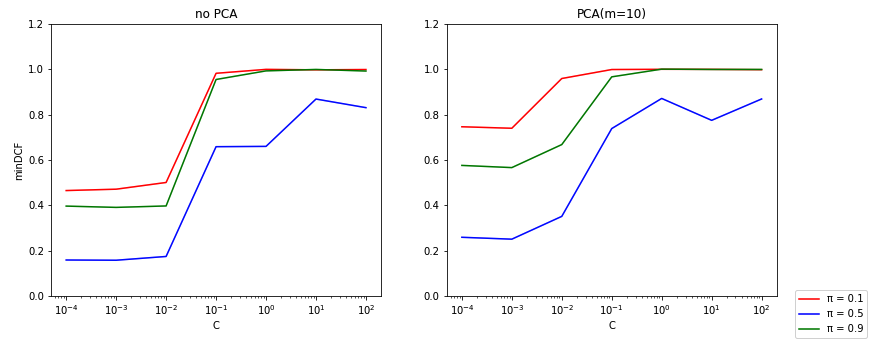
\includegraphics[width=\linewidth]{./Pictures/FeaturesAnalysis/polysvm.png}
	\caption{Polynomial SVM (K=1, c=1, d=2, raw features) - minDCF for different values of C}
	\label{polysvm} 
\end{figure}
The Polynomial Kernel SVM model was trained with raw features since the Z-Normalization step led to very poor results
for almost all the values of the hyperparameter $C$. 
By looking at figure \ref{polysvm} we can realize that the choice of $C$ is again
crucial and best performances are obtained for $C \le10^{-2}$. For this reason i have chosen 
$C=10^{-4}$ to show more detailed results.
% ---- POLYNOMIAL SVM TABLE ---
\FloatBarrier
\begin{table}[ht!]
	\centering
	\caption{Polynomial Kernel SVM - $C=10^{-4}$ - 3-fold cross validation}
	\begin{tabular}{ |l|l|l|l| }
		\hline
		& $\tilde{\pi}=0.1$ & $\tilde{\pi}=0.5$ & $\tilde{\pi}=0.9$ \\ \hline
		\multicolumn{4}{ |c| }{\bf{Raw features - no PCA}} \\
		\hline
		\multirow{2}{*}{}
		 Poly SVM \scriptsize{(c=0, d=2)}& 0.465 & 0.158 & 0.396\\
		 Poly SVM \scriptsize{(c=1, d=2)}& 0.187 & \textcolor{red}{0.060} & 0.164\\
		 Poly SVM \scriptsize{(c=1, d=3)}& 0.408 & 0.157 & \textcolor{blue}{0.563}\\
		\hline
		\multicolumn{4}{ |c| }{\bf{Raw features - PCA(m=11)}} \\
		\hline
		\multirow{2}{*}{}
		Poly SVM \scriptsize{(c=0, d=2)}& \textcolor{blue}{0.553} & 0.199 & 0.487\\
		Poly SVM \scriptsize{(c=1, d=2)}& 0.210 & \textcolor{red}{0.062} & \textcolor{orange}{0.158}\\
		Poly SVM \scriptsize{(c=1, d=3)}& 0.452 & 0.183 & 0.537\\
		\hline
		\multicolumn{4}{ |c| }{\bf{Raw features - PCA(m=10)}} \\
		\hline
		\multirow{2}{*}{}
		Poly SVM \scriptsize{(c=0, d=2)}& 0.746 & 0.258 & 0.576\\
		Poly SVM \scriptsize{(c=1, d=2)}& 0.465 & \textcolor{red}{0.158} & 0.396\\
		Poly SVM \scriptsize{(c=1, d=3)}& \textcolor{blue}{0.784} & 0.280 & \textcolor{blue}{0.815}\\
		\hline
	\end{tabular}
\end{table}
\FloatBarrier
% ---- POLYNOMIAL SVM CONSIDERATIONS ---
\begin{itemize}
	\item The Polynomial SVM is able to achieve better results with respect to some versions
		  of the Linear SVM. Best performances for the target application are achieved
		  by the model trained with $c=1$ and $d=2$.
	\item The use of PCA(m=11) helps in reducing the $minDCF$ for the $\tilde{\pi}=0.9$ application for the
		  model trained with $c=1$ and $d=2$ and doesn't affect that much the target application.
	\item PCA(m=10) led to worse performances in all the considered applications.
\end{itemize}
% ---- RBF SVM INTRO ---
The other kernel that was employed is the RBF kernel and these are the results achieved:
% ---- RBF SVM MINDCF PLOT ---
\begin{figure}[ht!]
	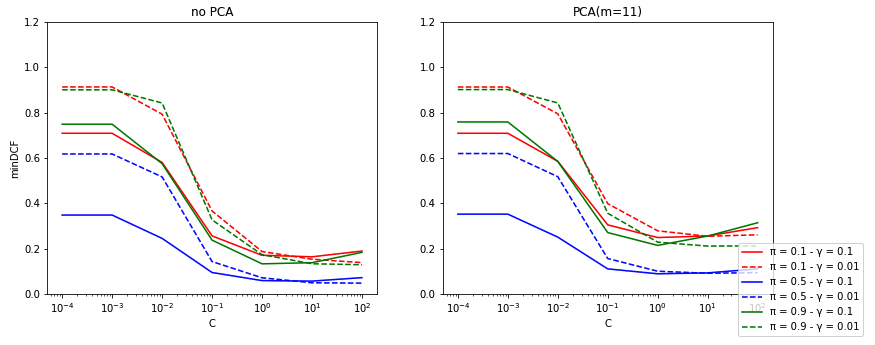
\includegraphics[width=\linewidth]{./Pictures/FeaturesAnalysis/rbfsvm_znorm_compl.png}
	\caption{RBF SVM ($K=1$, $\gamma \in \{0.1, 0.01\}$) - minDCF for different values of C}
	\label{rbfsvm_znorm} 
\end{figure}
In this case it was again used Z-normalization as pre-processing step. The hyperparameter $\gamma$ has to be tuned
so we trained the model for different values of $\gamma$ to analyze the performances and here are showed
the results for $\gamma = 0.1$ and $\gamma = 0.01$. Also the hyperparameter $C$ is still to be
chosed and needs to be estimated via cross-validation. The parameter $K$ has been set to $1$.
From figure \ref{rbfsvm_znorm} we again realize that the value of the hyperparameter $C$ is critical and we should choose a value
$C \ge 10^{-1}$. The table below shows the results obtained with $C=10$ and also results
obtained with $\gamma = 1$ appear for completeness.
\FloatBarrier
\begin{table}[ht!]
	\caption{RBF Kernel SVM - C=10}
	\centering
	\begin{tabular}{ |l|l|l|l| }
		\hline
		& $\tilde{\pi}=0.1$ & $\tilde{\pi}=0.5$ & $\tilde{\pi}=0.9$ \\ \hline
		\multicolumn{4}{ |c| }{\bf{Z-Normalized features - no PCA}} \\
		\hline
		\multirow{3}{*}{}
		 RBF SVM \scriptsize{($\gamma=1$)}& \textcolor{blue}{0.291} & 0.095 & 0.281\\
		 RBF SVM \scriptsize{($\gamma=0.1$)}& 0.163 & 0.056 & 0.137\\
		 RBF SVM \scriptsize{($\gamma=0.01$)}& 0.153 & \textcolor{red}{0.049} & 0.133\\
		\hline
		\multicolumn{4}{ |c| }{\bf{Z-Normalized features - PCA(m=11)}} \\
		\hline
		\multirow{3}{*}{}
		RBF SVM \scriptsize{($\gamma=1$)}& \textcolor{blue}{0.362} & 0.123 & 0.350\\
		RBF SVM \scriptsize{($\gamma=0.1$)}& 0.255 & 0.092 & 0.255\\
		RBF SVM \scriptsize{($\gamma=0.01$)}& 0.254 & \textcolor{red}{0.091} & 0.211\\
		\hline
		\multicolumn{4}{ |c| }{\bf{Z-Normalized features - PCA(m=10)}} \\
		\hline
		\multirow{3}{*}{}
		RBF SVM \scriptsize{($\gamma=1$)}& \textcolor{blue}{0.386} & 0.136 & 0.379\\
		RBF SVM \scriptsize{($\gamma=0.1$)}& 0.271 & \textcolor{red}{0.106} & 0.273\\
		RBF SVM \scriptsize{($\gamma=0.01$)}& 0.291 & 0.107 & 0.239\\
		\hline
	\end{tabular}
\end{table}
\FloatBarrier
% ---- BEST MODELS ---
\begin{table}[ht!]
	\caption{Best models analyzed up to now}
	\centering
	\begin{tabular}{ |l|l|l|l| }
		\hline
		& $\tilde{\pi}=0.1$ & $\tilde{\pi}=0.5$ & $\tilde{\pi}=0.9$ \\ \hline
		\multicolumn{4}{ |c| }{\bf{Gaussian Models}} \\
		\hline
		\multirow{2}{*}{}
		 Tied Cov \scriptsize{(Z-Norm, no PCA)}& 0.122 & 0.046 & 0.127\\
		 \hline
		 Tied Cov \scriptsize{(Gau, PCA(m=10))}& 0.212 & 0.082 & 0.207\\
		\hline
		\multicolumn{4}{ |c| }{\bf{Logistic Regression Models}} \\
		\hline
		\multirow{2}{*}{}
		LLR &&&\\\scriptsize{(Z-Norm, $\lambda = 10^{-6}$, no PCA)}& 0.132 & 0.047 & 0.126\\
		\hline
		QLR &&&\\\scriptsize{(Z-Norm, $\lambda = 10^{-5}$, no PCA)}& 0.153 & 0.052 & 0.142\\
		\hline
		\multicolumn{4}{ |c| }{\bf{SVM Models}} \\
		\hline
		LSVM &&&\\\scriptsize{(Z-Norm, $C=1$, no PCA)}& 0.129 & 0.047 & 0.130\\
		\hline
	\end{tabular}
\end{table}
% ---- RBF SVM CONSIDERATIONS ---
\begin{itemize}
	\item RBF kernel version of the SVM achieves results that are near to the ones
		  obtained with the linear version and behaves better w.r.t. the Polynomial
		  version
	\item The most promising value of $\gamma$ seems to be $\gamma=0.01$ because with this
		  value we are able to obtain the best $minDCF$ for the target application (when no
		  PCA is applied)
	\item PCA is not able to provide any better results in terms of $minDCF$
\end{itemize}
% ---- KERNEL SVM COMPARISON ---
\textit{Comparison}: The linear version of the SVM achieves better results with
respect to the two kernel versions. This is aligned with the fact that also in Logistic Regression
linear model worked better.
\underline{Selected Kernel SVM Models}:
\begin{itemize}
	\item Polynomial SVM: Raw features, $K=1$, $C=10^{-4}$, $c=1$, $d=2$, PCA(m=11)
	\item RBF SVM: Z-Normalized features, $K=1$, $C=10$, $\gamma=0.01$, no PCA
\end{itemize}
%--
%%%%%%%%%%%%%%%%%%%%%%%%%%%%%%%%%%%%%%%%%%%%%%%%%%%%%%%%%%%%
%%%%%%%%%%%%%%%%%%%%%% GMM	 CLASSIFIER %%%%%%%%%%%%%%%%%%%%
%%%%%%%%%%%%%%%%%%%%%%%%%%%%%%%%%%%%%%%%%%%%%%%%%%%%%%%%%%%%
\subsection{GMM Classifier}
The last model we are going to take into account is a generative model. 
The GMM problem is related to the estimation of a population distribution and can be 
also applied to the classification task. We resort the class-posterior probability
used for the Gaussian classifiers:
\begin{center}
	$f_X(x) = \sum_{c=1}^K f_{X|C}(x|c) \cdot P(C=c) = \sum_{c=1}^K \mathcal{N}(x|\mu_c,\Sigma_c) \cdot \pi_c$
\end{center}
more in general we can introduce a weight term instead if the prior probability that will
be one of the model paramers of the GMM:
\begin{center}
	$X \sim GMM(M,\mathcal{S},w) \Rightarrow f_X(x) = \sum_{g=1}^M w_g \cdot \mathcal{N}(x|\mu_g,\Sigma_g)$
\end{center}
so the GMM density is the sum of $M$ Gaussians where 
$M=[\mu_1,...,\mu_M], \mathcal{S}=[\Sigma_1,...,\Sigma_M], w=[w_1,...,w_M]$ are the
model parameters. Gaussian components can be seen as clusters the samples belog to (in
a hard or in a soft way) and the cluster label is a latent random variable. If we define
\begin{center}
	$f_{X_i,G_i}(x_i,g)=w_g\mathcal{N}(x_i|\mu_g,\Sigma_g)$ and \\
	$f_{X_i}(x_i) = \sum_{g=1}^M f_{X_i,G_i}(x_i,g)$
\end{center}
we can introduce a term called \textit{responsability} that represents the posterior probability
that a sample belongs to a certain cluster(component):
\begin{center}
	$\gamma_{g,i} = P(G_i = g|X_i=x) = \frac{f_{X_i,G_i}(x_i,g)}{f_{X_i}(x_i)} = \frac{w_g\mathcal{N}(x_i|\mu_g,\Sigma_g)}{\sum_{g'} w_{g'}\mathcal{N}(x_i|\mu_{g'},\Sigma_{g'})}$
\end{center}
We can assign the sample to the cluster label for which the responsability is maximum and 
then re-estimate the model parameters given the cluster assignments. An evident
problem is that we are forming hard clusters so we are not admitting that a sample could
belong to more than one cluster(component). To handle soft-clusters we introduce the statistics:
\begin{center}
		$F_g=\sum_{i=1}^N \gamma_{g,i}x_i$, \;$S_g=\sum_{i}\gamma_{g,i}x_ix_i^T$, \;$N_g=\sum_{i=1}^N \gamma_{g,i}$
\end{center}
to obtain a re-estimate of $w_g = \frac{N_g}{N}$.
In this way we will be able to apply the Expectation-Maximization algorithm:
\begin{itemize}
	\item E-step: estimate (given the model parameters $(M_t,\mathcal{S}_t,w_t)$):
			\begin{center}
				$\gamma_{g,i}=P(G_i=g|C_i=x,M_t,\mathcal{S}_t,w_t)$ 
			\end{center}
	\item M-step: estimate the new model parameters by usign the statistics mentioned above
\end{itemize}
The estimation goes on starting from an initial value of the model parameters until a certain
criterion is met. The EM algorithm thus require an initial estimate for the GMM parameters so
we employ the LBG algorithm to incrementally construct a  GMM with $2G$ componenets from a 
GMM with $G$ components. The starting point will be $(1, \mu, C)$ so we use the empirical
mean and covariance matrix of the dataset. We can then build a 2-componenents model starting from
a single one and from each of the new componenets we generate other new 2 componenets and so on and so forth.
\\We are also going to introduce a Diagonal and Tied version of the GMM problem: the diagonal
variant consists of a model where each component has a diagonal covariance matrix (this does
not correspond with the Naive Bayes assumption did for the Gaussian models). The Tied covariance
model assumes that the covariance of a single GMM $\Sigma_{c,g} = \Sigma_c$ are the same but
each GMM of each class has a difference covariance matrix $\Sigma_c$ (again, this is different
from the Tied MVG model).

We are now going to train a GMM
over the samples of each class. Given the fact that almost all the features are already well
distributed according to the Gaussian hypothesis i suppose that we won't need many gaussian 
components for the model. Moreover, Tied GMM model is supposed to outperform the other two
models as already seen in the Gaussian classifiers.
\begin{figure}[ht!]
	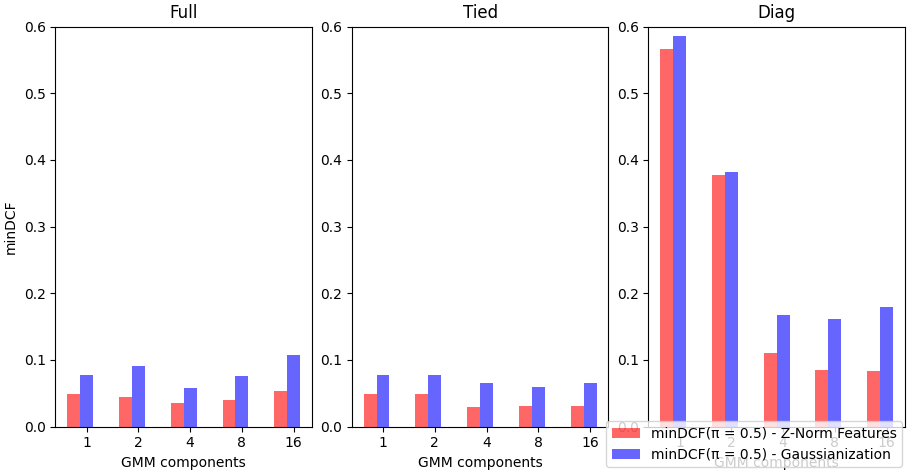
\includegraphics[width=\linewidth]{./Pictures/FeaturesAnalysis/gmmhist.png}
	\caption{GMM - minDCF for different number of components}
	\label{gmmhist} 
\end{figure}
By considering only models trained with 8 compoents we are now going to show 
more in detail the results obtained when training with and without PCA.
\begin{table}[ht!]
	\caption{GMM - 3-fold cross validation}
	\centering
	\begin{tabular}{ |l|l|l|l| }
		\hline
		& $\tilde{\pi}=0.1$ & $\tilde{\pi}=0.5$ & $\tilde{\pi}=0.9$ \\ \hline
		\multicolumn{4}{ |c| }{\bf{Z-normalized features - no PCA}} \\
		\hline
		\multirow{3}{*}{}
		 GMM Full (8 comp.)& 0.109 & 0.040 & 0.102\\
		 GMM Tied (8 comp.)& 0.099 & \textcolor{red}{0.031} & 0.075\\
		 GMM Diag (8 comp.)& 0.214 & 0.085 & \textcolor{blue}{0.215}\\
		\hline
		\multicolumn{4}{ |c| }{\bf{Z-normalized features - PCA(m=11)}} \\
		\hline
		\multirow{3}{*}{}
		GMM Full (8 comp.)& 0.229 & 0.074 & 0.175\\
		GMM Tied (8 comp.)& 0.198 & \textcolor{red}{0.067} & 0.166\\
		GMM Diag (8 comp.)& \textcolor{blue}{0.311} & 0.111 & 0.275\\
		\hline
		\multicolumn{4}{ |c| }{\bf{Z-normalized features - PCA(m=10)}} \\
		\hline
		\multirow{3}{*}{}
		GMM Full (8 comp.)& \textcolor{orange}{0.225} & 0.082 & 0.212\\
		GMM Tied (8 comp.)& 0.204 & \textcolor{red}{0.072} & 0.186\\
		GMM Diag (8 comp.)& \textcolor{blue}{0.310} & \textcolor{orange}{0.108} & \textcolor{orange}{0.260}\\
		\hline
		\multicolumn{4}{ |c| }{\bf{Gaussianized features - no PCA}} \\
		\hline
		\multirow{3}{*}{}
		GMM Full (8 comp.)& 0.221 & 0.076 & 0.210\\
		GMM Tied (8 comp.)& 0.158 & \textcolor{red}{0.059} & 0.151\\
		GMM Diag (8 comp.)& \textcolor{blue}{0.419} & 0.162 & 0.397\\
		\hline
		\multicolumn{4}{ |c| }{\bf{Gaussianized features - PCA(m=11)}} \\
		\hline
		\multirow{3}{*}{}
		GMM Full (8 comp.)& 0.246 & 0.091 & \textcolor{orange}{0.199}\\
		GMM Tied (8 comp.)& 0.175 & \textcolor{red}{0.066} & 0.169\\
		GMM Diag (8 comp.)& 0.477 & 0.174 & \textcolor{blue}{0.415}\\
		\hline
		\multicolumn{4}{ |c| }{\bf{Gaussianized features - PCA(m=10)}} \\
		\hline
		\multirow{3}{*}{}
		GMM Full (8 comp.)& 0.274 & 0.096 & 0.257\\
		GMM Tied (8 comp.)& 0.185 & \textcolor{red}{0.069} & 0.185\\
		GMM Diag (8 comp.)& \textcolor{orange}{0.406} & \textcolor{orange}{0.148} & \textcolor{orange}{0.356}\\
		\hline
	\end{tabular}
\end{table}
\begin{itemize}
	\item As showed in figure \ref{gmmhist}, for a relative small number of components (8) good results are
	achieved by all the three types of models.
	\item Even if diag assumption doesn't hold really well
	especially when the number of components is low it performs better with higher number of 
	components.
	\item  The Tied model is the one with best results even if the Full model still performs really
	well and this corresponds to the hypothesis made before according to what has already been
	 analyzed for the Gaussian models.
	\item Gaussianization never helps in achieving better results. According to what we
	had seen with the MVG models the already good distribution of data makes this classification
	task not benefitting from the Gaussianization pre-processing step and worse results are achieved
	when it is applied.
	\item PCA is not helpful in achieving better results (we can see an improvements for some
	applications when PCA(m=10) is applied w.r.t to PCA(m=11) but all these results are worse
	w.r.t the no PCA versions of the trained models). With Gaussianization and PCA(m=11) instead
	we can notice an improvement for $\tilde{\pi}=0.9$ application.
\end{itemize}
\begin{table}[ht!]
	\caption{Best models analyzed up to now}
	\centering
	\begin{tabular}{ |l|l|l|l| }
		\hline
		& $\tilde{\pi}=0.1$ & $\tilde{\pi}=0.5$ & $\tilde{\pi}=0.9$ \\ \hline
		\multicolumn{4}{ |c| }{\bf{Gaussian Models}} \\
		\hline
		\multirow{2}{*}{}
		 Tied Cov \scriptsize{(Z-Norm, no PCA)}& 0.122 & 0.046 & 0.127\\
		 Tied Cov \scriptsize{(Gau, PCA(m=10))}& 0.212 & 0.082 & 0.207\\
		\hline
		\multicolumn{4}{ |c| }{\bf{Logistic Regression Models}} \\
		\hline
		\multirow{2}{*}{}
		LLR &&&\\\scriptsize{(Z-Norm, $\lambda = 10^{-6}$, no PCA)}& 0.132 & 0.047 & 0.126\\
		\hline
		QLR &&&\\\scriptsize{(Z-Norm, $\lambda = 10^{-5}$, no PCA)}& 0.153 & 0.052 & 0.142\\
		\hline
		\multicolumn{4}{ |c| }{\bf{SVM Models}} \\
		\hline
		LSVM &&&\\\scriptsize{(Z-Norm, no PCA)}& 0.129 & 0.047 & 0.130\\
		Poly SVM &&&\\\tiny{(Raw, $c=1$, $d=2$, PCA(m=11))}& 0.210 & 0.062 & 0.158\\
		RBF SVM &&&\\\scriptsize{(Z-Norm, $\gamma = 0.01$, no PCA)}& 0.153 & 0.049 & 0.133\\
		\hline
	\end{tabular}
\end{table}
The GMM Tied(8 components) trained with Z-Normalization and no PCA is the one that achieves
the best results among all the models evaluated up to now.\\
\underline{Selected GMM Model}:
\begin{itemize}
	\item GMM Tied (8 componenets), Z-Normalization, no PCA
\end{itemize}
%%%%%%%%%%%%%%%%%%%%%%%%%
%%% SCORE CALIBRATION %%%
%%%%%%%%%%%%%%%%%%%%%%%%%
\section{Score Calibration}
\subsection{Calibration Analysis On Selected Models}
We now select one candidate for each of the previous analyzed classification models (Gaussian, Logisti Regression,
SVM, GMM):
\begin{itemize}
	\item \underline{Gaussian model}: Tied-Cov (Z-Normalization, no PCA)
	\item \underline{Logistic Regression}: Linear LR (Z-Normalization, no PCA)
	\item \underline{SVM}: Linear SVM (Z-Normalization, no PCA)
	\item \underline{GMM}: Tied GMM with 8 components (Z-normalization, no PCA)
\end{itemize}
% Bayes error plot
% Comment on Bayes error plot
\subsection{Calbrating Scores For Selected Models}
We are going to transform the scores provided by each model so that the theoretical threshold $t = -log\;\frac{\tilde{\pi}}{1-\tilde{\pi}}$
provides close to optimal values over a wide range of effective priors $\tilde{\pi}$. What we want to find is a 
monotonic function $f$ that maps not-calibrated scores in calibrated scores.\\
We assume that the function $f$ has the form:
\begin{center}
	$f(s) = \alpha s + \beta$
\end{center}
and $f(s)$ can be interpreted as log-likelihood ratio for the two classes hypotheses:
\begin{center}
	$f(s) = log\;\frac{f_{S|C}(s|\mathcal{H}_T)}{f_{S|C}(s|\mathcal{H}_F)} = \alpha s + \beta$
\end{center}
and the class posterior probabilty for prior $\tilde{\pi}$ corresponds to:
\begin{center}
	$log\;\frac{P(C=\mathcal{H}_T|s)}{P(C=\mathcal{H}_F|s)} = \alpha s + \beta + log\;\frac{\tilde{\pi}}{1-\tilde{\pi}}$
\end{center}
By interpreting scores $s$ as samples of a dataset (where each sample has 1 feature) we can employ a prior weighted
logistic regression model to learn the model parameters over our calibration set (the dataset composed of the
scores for a certain model). If we let:
\begin{center}
	$\beta' = \beta + log\;\frac{\tilde{\pi}}{1-\tilde{\pi}}$
\end{center}
we have exactly a Logistic Regression model where $\alpha$ and $\beta'$ are the model parameters we have to learn.
We have still to specify a prior $\tilde{\pi}$ that will be the one of our target application even if we will notice
that the improvements in terms of calibration will also involve the unbalanced applications. To obtain calibrated
scores we will have to compute:
\begin{center}
	$f(s) = \alpha s + \beta = \alpha s + \beta' - log\;\frac{\tilde{\pi}}{1-\tilde{\pi}}$
\end{center}
\begin{figure}[ht!]
	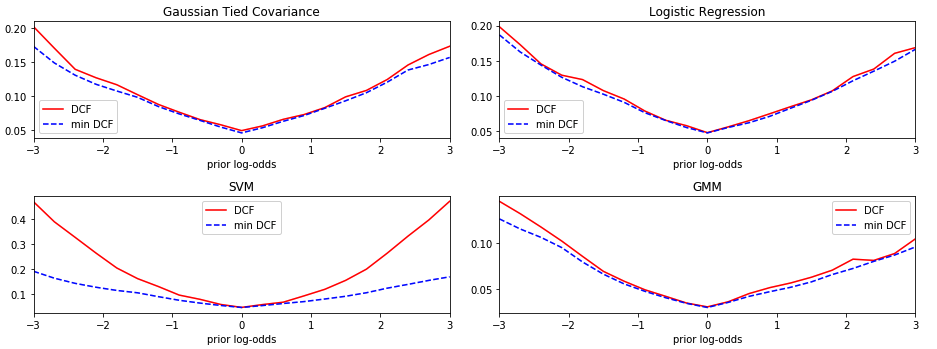
\includegraphics[width=\linewidth]{./Pictures/FeaturesAnalysis/bestmodels_nc.png}
	\caption{Bayesian Error Plots for each of the selected models (without score calibration)}
	\label{bayesianerrornotcalibrated} 
\end{figure}
The Tied Gaussian, Linear Logistic Regression and Tied GMM models seem to be already well calibrated
in particular for positive values of the prior log-odds. The Tied Gaussian model
could be slightly improved in terms of calibration for negative values
of the prior log odds. The SVM instead is not well calibrated for almost every
considered values of the prior log-odds.
\begin{figure}[ht!]
	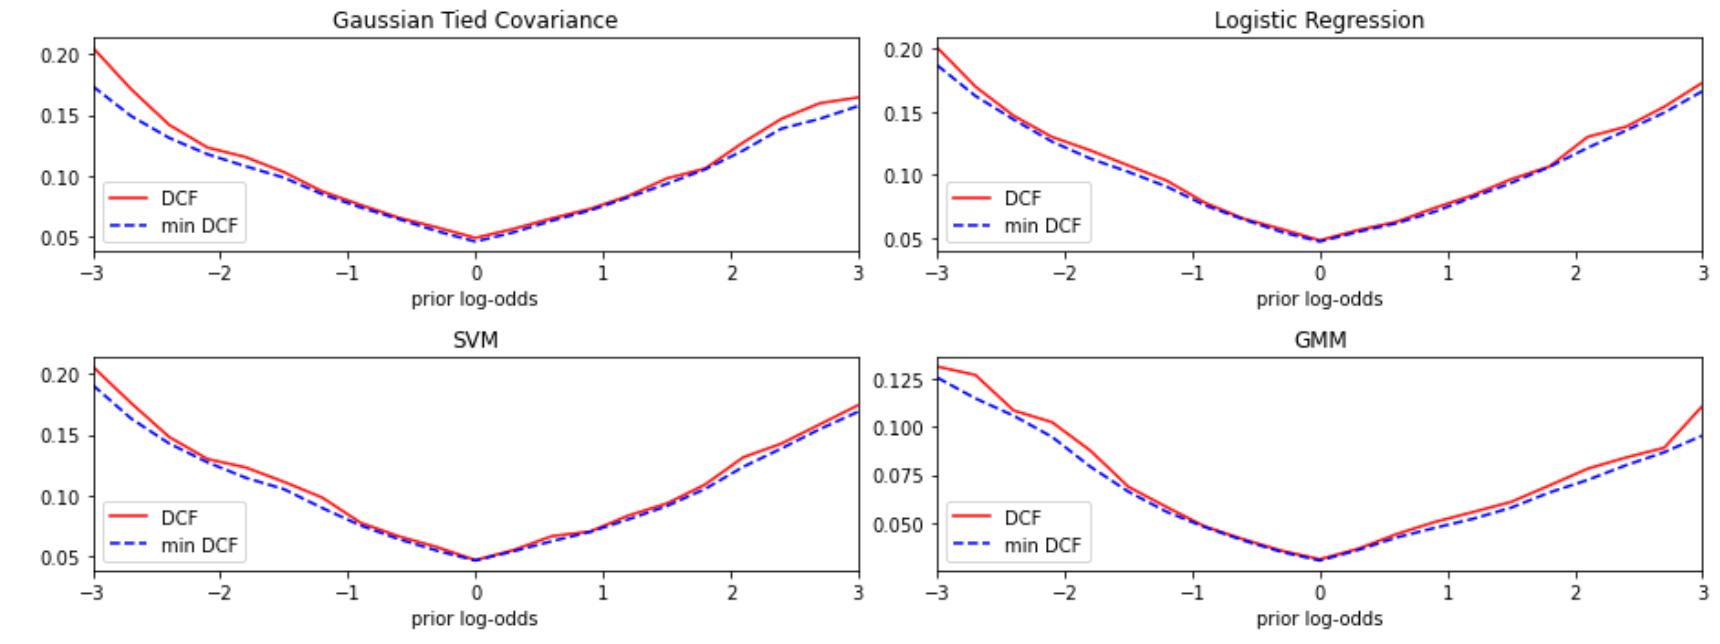
\includegraphics[width=\linewidth]{./Pictures/FeaturesAnalysis/bestmodels_c.png}
	\caption{Bayesian Error Plots for each of the selected models (with score calibration)}
	\label{bayesianerrorcalibrated} 
\end{figure}
\FloatBarrier
\begin{table}[ht!]
	\caption{Calibrated vs not calibrated scores for best selected models}
	\centering
	\begin{tabular}{ |l|l|l|l| }
		\hline
		& $\tilde{\pi}=0.1$ & $\tilde{\pi}=0.5$ & $\tilde{\pi}=0.9$ \\ \hline
		\multicolumn{4}{ |c| }{\bf{Uncalibrated scores [minDCF / DCF]}} \\
		\hline
		\multirow{4}{*}{}
		 \small{Tied Gaussian} & \footnotesize{0.122/0.127} & \footnotesize{0.046/0.050} & \footnotesize{0.127/0.134}\\
		 \small{Lnear LR} & \footnotesize{0.132/0.139} & \footnotesize{0.047/0.048} & \footnotesize{0.126/0.136}\\
		 \small{Linear SVM} & \footnotesize{0.132/0.289} & \footnotesize{0.047/0.047} & \footnotesize{0.129/0.285}\\
		 \small{Tied GMM} & \footnotesize{0.099/0.110} & \footnotesize{0.031/0.031} & \footnotesize{0.075/0.081}\\
		\hline
		\multicolumn{4}{ |c| }{\bf{Calibrated scores [minDCF / DCF]}} \\
		\hline
		\multirow{4}{*}{}
		\small{Tied Gaussian} & \footnotesize{0.122/\textcolor{red}{0.128}} & \footnotesize{0.046/\textcolor{green}{0.049}} & \footnotesize{0.127/\textcolor{red}{0.135}}\\
		\small{Lnear LR} & \footnotesize{0.132/\textcolor{red}{0.141}} & \footnotesize{0.047/0.048} & \footnotesize{0.126/\textcolor{green}{0.132}}\\
		\small{Linear SVM} & \footnotesize{0.132/\textcolor{green}{0.135}} & \footnotesize{0.047/0.047} & \footnotesize{0.129/\textcolor{green}{0.137}}\\
		\small{Tied GMM} & \footnotesize{0.099/\textcolor{green}{0.105}} & \footnotesize{0.031/0.031} & \footnotesize{0.075/\textcolor{green}{0.076}}\\
		\hline
	\end{tabular}
\end{table}
\FloatBarrier
We can easily notice that for models where scores where already well calibrated the score
calibration didn't provide effective benefits (in some cases we also obtained
slightly worse results). For SVM model great benefits are obtained for the unbalanced
applications.
\section{Experimental Results}
Now we are going to train all the previous models on the entire training set and the 
evaluation set will be used for the first time to assest if the results obtained so far
are consistent and the best model selected is confirmed (we could also realize that
other choices would have been better for this evaluation set).
\FloatBarrier
\begin{table}[ht!]
	\caption{minDCF over evaluation set for all models trained over the whole training set (Z-Normalized features, no PCA)}
	\centering
	\begin{tabular}{ |l|l|l|l| }
		\hline
		& $\tilde{\pi}=0.1$ & $\tilde{\pi}=0.5$ & $\tilde{\pi}=0.9$ \\ \hline
		\multicolumn{4}{ |c| }{\bf{Gaussian Models (Z-normalized features, no PCA)}} \\
		\hline
		\multirow{3}{*}{}
		 Full Cov & 0.134 & 0.053 & 0.138 \\
		 Tied Cov & 0.133 & 0.051 & 0.135 \\
		 Naive Bayes & 0.810 & 0.570 & 0.882 \\
		\hline
		\multicolumn{4}{ |c| }{\bf{LR Models (Z-Normalized features, no PCA)}} \\
		\hline
		\multirow{2}{*}{}
		LLR \scriptsize{($\lambda = 10^{-6}$)} & 0.135 & 0.052 & 0.133 \\
		QLR \scriptsize{($\lambda = 10^{-5}$)} & 0.148 & 0.053 & 0.141 \\
		\hline
		\multicolumn{4}{ |c| }{\bf{SVM Models (Z-Normalized features, no PCA)}} \\
		\hline
		\multirow{2}{*}{}
		LSVM &&&\\\scriptsize{($K=0, C=1$)} & 0.142 & 0.052 & 0.137 \\
		Poly SVM &&&\\\scriptsize{($K=1, C=10^{-4}, c=1, d=2$)} & 0.194 & 0.062 & 0.163 \\
		RBF SVM &&&\\\scriptsize{($K=1, C=10, \gamma=0.01$)} & 0.138 & 0.054 & 0.133 \\
		\hline
		\multicolumn{4}{ |c| }{\bf{GMM Models (Z-Normalized features, no PCA)}} \\
		\hline
		\multirow{6}{*}{}
		GMM Full (8 comp.) & 0.092 & 0.034 & 0.086 \\
		GMM Full (16 comp.) & 0.103 & 0.043 & 0.117 \\
		GMM Tied (8 comp.) & 0.088 & 0.030 & 0.087 \\
		GMM Tied (16 comp.) & 0.089 & 0.033 & 0.086 \\
		GMM Diag (8 comp.) & 0.236 & 0.090 & 0.234 \\
		GMM Diag (16 comp.) & 0.244 & 0.098 & 0.232 \\
		\hline
	\end{tabular}
\end{table}
\FloatBarrier
\begin{table}[ht!]
	\caption{minDCF over evaluation set for all models trained over the whole training set (Z-Normalized features, PCA(m=11))}
	\centering
	\begin{tabular}{ |l|l|l|l| }
		\hline
		& $\tilde{\pi}=0.1$ & $\tilde{\pi}=0.5$ & $\tilde{\pi}=0.9$ \\ \hline
		\multicolumn{4}{ |c| }{\bf{Gaussian Models (Z-normalized features, PCA(m=11))}} \\
		\hline
		\multirow{3}{*}{}
		 Full Cov & 0.280 & 0.113 & 0.255 \\
		 Tied Cov & 0.278 & 0.111 & 0.256 \\
		 Naive Bayes & 0.293 & 0.116 & 0.263 \\
		\hline
		\multicolumn{4}{ |c| }{\bf{LR Models (Z-Normalized features, PCA(m=11))}} \\
		\hline
		\multirow{2}{*}{}
		LLR \scriptsize{($\lambda = 10^{-6}$)} & 0.281 & 0.110 & 0.259 \\
		QLR \scriptsize{($\lambda = 10^{-5}$)} & 0.253 & 0.108 & 0.258 \\
		\hline
		\multicolumn{4}{ |c| }{\bf{SVM Models (Z-Normalized features, PCA(m=11))}} \\
		\hline
		\multirow{2}{*}{}
		LSVM &&&\\\scriptsize{($K=0, C=1$)} & 0.277 & 0.110 & 0.262 \\
		Poly SVM &&&\\\scriptsize{($K=1, C=10^{-4}, c=1, d=2$)} & 0.189 & 0.068 & 0.151 \\
		RBF SVM &&&\\\scriptsize{($K=1, C=10, \gamma=0.01$)} & 0.243 & 0.109 & 0.246 \\
		\hline
		\multicolumn{4}{ |c| }{\bf{GMM Models (Z-Normalized features, PCA(m=11))}} \\
		\hline
		\multirow{6}{*}{}
		GMM Full (8 comp.) & 0.179 & 0.080 & 0.196 \\
		GMM Full (16 comp.) & 0.219 & 0.086 & 0.211 \\
		GMM Tied (8 comp.) & 0.173 & 0.072 & 0.195 \\
		GMM Tied (16 comp.) & 0.185 & 0.078 & 0.194 \\
		GMM Diag (8 comp.) & 0.329 & 0.124 & 0.312 \\
		GMM Diag (16 comp.) & 0.311 & 0.141 & 0.327 \\
		\hline
	\end{tabular}
\end{table}
The results obtained by training the models on the entire training set and by evaluating
them on the entire evaluation set are coherent with the results previously
obtained and with the observations made. The ROC curve in figure \ref{roc} shows (and confirms) that the best performing model is the Tied GMM with 8 componenets. 
The other three models also perform really well but slightly worse than this.
\begin{figure}[ht!]
	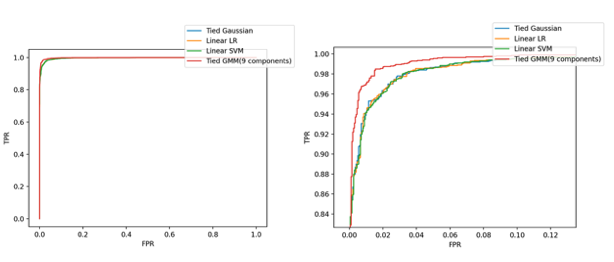
\includegraphics[width=\linewidth]{./Pictures/FeaturesAnalysis/roc.png}
	\caption{ROC curves of selected models (on the right a zoomed version)}
	\label{roc} 
\end{figure}
\section{Conclusions}
We can conclude by saying that in general linear models have better performances
on these data with respect to the non-linear ones. Due to the high level of correlation
among features the PCA didn't help in achieving better results (despite  the fact that with PCA(m=11)
we have obtained not a big performance degratation in most of the models) and Naive hypothesis didn't worked
well in Gaussian models. We have been able to reach a $minDCF\approx0.03$ for
the target application($\tilde{\pi}=0.5$) but also for the unbalanced applications
we were able to achieve good results ($minDCF\approx0.1$ for $\tilde{\pi}=0.1$ and 
$minDCF\approx0.1$ for $\tilde{\pi}=0.9$). The choices made on the training set
via k-fold cross-validation proved to be coherent with the results obtained on
the entire training set.
%----------------------------------------------------------------------------------------
%	BIBLIOGRAPHY
%----------------------------------------------------------------------------------------

\printbibliography[title={Bibliography}] % Print the bibliography, section title in curly brackets

%----------------------------------------------------------------------------------------

\end{document}
